\chapter{Results, Conclusion and outlook}
In this chapter we will present the results achieved and draw final conclusions.
The chapter ends with an outlook on possible directions to continue and improve
the work done so far.

\section{Results}
Here we will present hopefully the interesting results achieved \dots

Bla bla bla

more bla bla bla

For the final analysis a set of classroom profiles have been selected

\begin{itemize}
    \item \textbf{Class A:} Description
    \item \textbf{Class B:} ...
    \item \textbf{Class C:} ...
\end{itemize}

Comparing those classroom profile produces the following HA-Plot

\begin{figure}[H]
    \makebox[\textwidth][l]{%
    \begin{minipage}[t]{500pt}
        \centering
        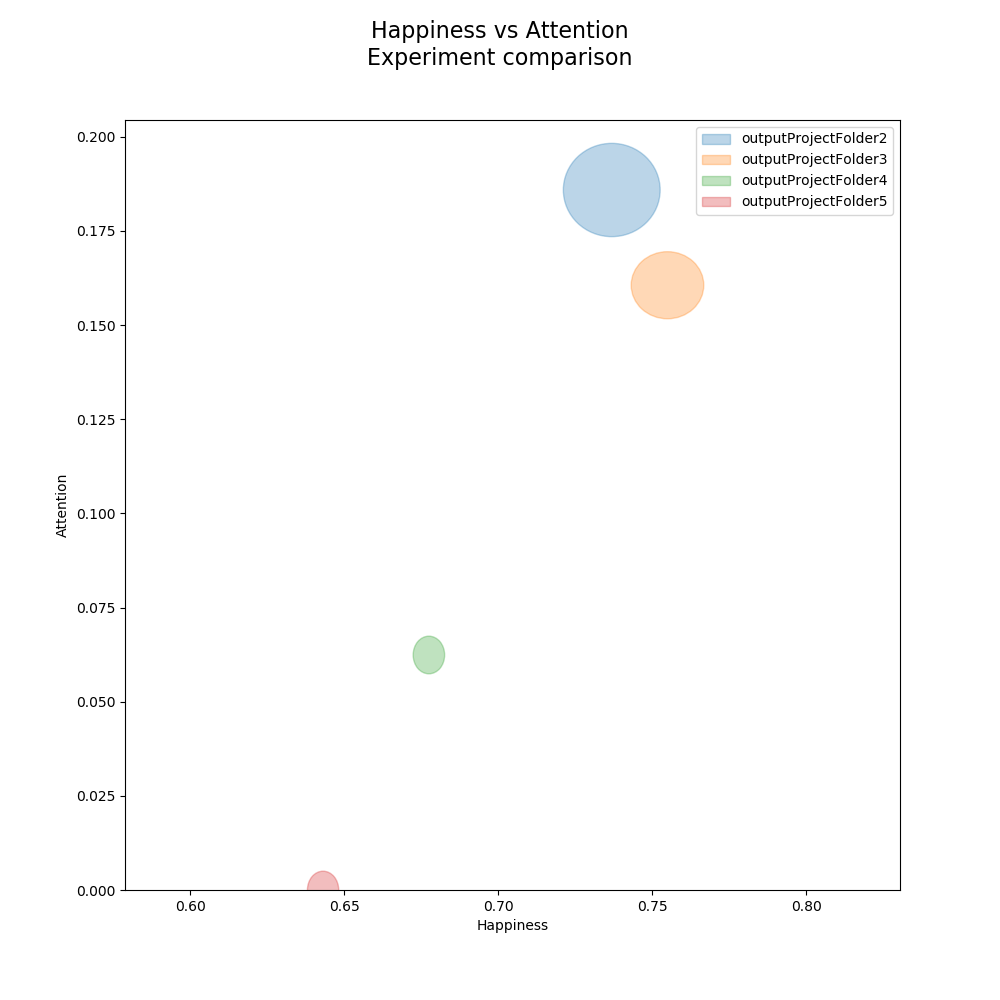
\includegraphics[width=400pt]{StudyResults}
        \caption{Final Study results}
        \label{StudyResults}
    \end{minipage}    
    }%
\end{figure}

This result can be interpreted to be ....

Bla bla bla

\dots


\section{Conclusion}
As part of the thesis we have developed a multi-agent model that is simulation a virtual classroom.

We have devised a Agent Logic that is based on the established Big-Five Personality
Trait model and that produces agent behavior consistent with empirical studies.

We have developed a data analysis pipeline that makes it possible to efficiently
run multiple simulations in a batch mode, enabling a statistical analysis of the
simulation results.

Based on the pedagogical literature about classroom dynamics we have selected a
set of interesting classroom profiles and compared their simulation results.

Doing so we found that \dots bla bla bla results

The simulation software, the data analysis scripts and all content presented in this
thesis is available freely under the MIT License from the github repository \href{https://github.com/mapa17/breakfastclub}{https://github.com/mapa17/breakfastclub}.



\section{Outlook}
As mentioned shortly in the chapter on Objectives some initial objectives had to
be dropped during the development of the thesis in order to stay within the available
time frame.

The following is a list of possible improvements, as well as ideas for follow up projects.

\begin{itemize}
    \item \textbf{Interactive Simulation:} 
    On way to extend the how the simulation can be used, is to make the simulation
    interactive. Doing so would provide the user with the option to force agents
    to perform certain actions, expulse students from the classroom, call for silence
    or similar interactions. This would make it possible to develop a teacher training 
    program, based on the simulator, similar to commercial solutions like TLE TeachLive
    \cite{Dieker2017} or simSchool \cite{Badiee2015} but open source and with
    agent behavior that is based on a psychological model.
    
    \bb
    
    In order to support learning and provide a novel visualization of the effect
    of user interaction with the simulation we envisioned a system that is able to track
    the effect of each user interaction onto the final result of the simulation.
    This could be achieved by creating a clone of the running simulation when ever
    the user is performing an action. That clone instance would continue until the 
    end of the simulation unperturbed, and could be compared to the all other clones
    generated in the same way. This would make it possible to evaluate the effect
    of each user interaction onto the final result of the simulation, and visualize it
    as a trace instead of a dot in the HA-Plot.

    \item \textbf{Reinforcement trained teacher:} At the moment the simulation
    is consisting of only students that behave like an autonomous study group.
    With the teacher interactions described in the previously, one could train a
    virtual teacher using reinforcement learning (RL) with
    the objective to maximize happiness and attention of the class.
    
    \bb

    As there is a fast amount of literature on different teaching methodologies,
    it would be interesting to study if the RL trained teacher applies any of the known
    methodologies or applies new ones. Another interesting aspect would be to study the
    effect different classroom profiles have on the trained teacher, with other
    word, how different classroom profiles form and shape teacher behavior.

    \item \textbf{Screening of classroom profiles:} One obvious extension based
    on the batch processing capabilities of the simulation is to perform a kind
    of screening studying. One would systematically evaluate a high number of personality
    profiles, similar to screening studies in Bioinformatics, comparing thousands
    of combination in order to find interesting tipping points, extremes and curious
    singularities.

    \item \textbf{Dominance hierarchy:} The current simulation when calculating
    the peer pressure on a individual agent is modeling a flat social hierarchy.
    One could extend this to a more realistic Dominance Hierarchy, giving different
    agents different weights in controlling the classroom interest. Such a Dominance
    hierarchy in place one could extend its effect on other actions like chat or
    quarrel, making the outcome of interactions depend as well on the position
    of agents in the dominance hierarchy.

    \item \textbf{Learning Agents:} Because of simplicity the agents have no capability
    to learn and adapt their behavior over time. One could prevent some simple learning
    mechanisms, that would open a wide range of new questions one can study, concerning
    the dynamics of agent and group behavior over longer durations of time.
\end{itemize}

\section{Acknowledgement}
We especially want to thank Prof. Dr. Michael Kickmeier-Rust for this continuos
support and mentoring. Without him this work would have not been possible.
